\chapter{Introduction}
This thesis is based on part of the EPI-project, developed at Barcelona Supercomputing Center, in particular on the V-Extension implementation.
In this Chapter all the RISC-V and V-Extension concepts will be presented and discussed, but not all of the topics regarding the RISC-V ISA or all the extensions are relevant to the project, so they will not be presented.\\
Beginning with the Concepts there will also be an explaination on the context of the project, so the real implementation and application of the ISA specifications.
With a particular focus on Verification concepts and on the UVM structure, filled by the details useful to understand the work done.



\section{Concepts}
\subsection{RISC-V}
RISC-V is an open, extensible and free instruction set architecture (ISA). It was designed solely to support computer architecture research and education\cite{RISC-V-Instruction-Set-Manual}.\\
The project, began at the Berkley, University of California in 2010, published the first ISA User Manual in 2011. Afterward that there was the first tapeout of a RISC-V chip in 28nm FDSOI donated by STMicroelectronics.\\

The RISC-V ISA is implemented as a base integer ISA, but it is modular and so supports  variable-length instruction encodings.\\
This ISA is provided under open source licenses, and it is gaining a lot of popularity due to its open nature. \\
Mainly there are two primary base integer variants, RV32I and RV64I, which provide 32-bit or 64-bit user-level address spaces respectively.\\

\subsubsection{Extensions}

RISC-V is designed to have a good customization which is the reason why it is provided with the possibility to be extended, but the base integer instructions cannot be redefined.\\
There are two kinds of extensions:
\textit{standard} and \textit{non-standard}.
\begin{itemize}
    \item The \textit{standard} ones need to be compatible with all the other standards and they should also aim to be generally useful.
    \item The \textit{non-standard} ones can be highly specialized in some task and therefore they may conflict with other extensions.
\end{itemize}

For general development some standard extensions are predefined:
\begin{itemize}
    \item "\textbf{I}" is the base integer extension and contains integer computational instructions, integer loads, integer stores, and control-flow instructions. It is mandatory for all RISC-V implementations.
    
    \item "\textbf{M}" is the standard integer multiplication and division extension, it allows to multiply and divide the values held in the integer registers.
    
    \item "\textbf{A}" is the standard atomic instruction extension. It is useful to have atomic instructions for inter-processor synchronization. In fact, with this extension is possible to read, modify, and write memory atomically. 
    
    \item "\textbf{F}" is the standard single-precision floating-point extension. It adds floating-point registers, single-precision computational instructions, and single-precision loads and stores. 
    
    \item "\textbf{D}" The standard double-precision floating-point extension. Advantageous when the F extension is not enough, it expands the extension and adds double-precision computational instructions, loads, and stores.
    
    \item "\textbf{G}" is the denotation for an integer base plus these four standard extensions (“IMAFD”).
\end{itemize}


The design philosophy of the RISC-V projects is based on modularity: the base ISA will not change over time, but new extensions will be available and new feature will be added. This is useful because is very difficult to find general useful extension beyond the ones already exist. So it wouldn't be convenient to constantly add new features to the base ISA and then have to keep track of that.\\

\subsubsection{Base instructions}
In Figure \ref{riscv-base-instruction-formats} it is possible to see how the base instruction are composed.

\begin{figure}[H]
    \centering
    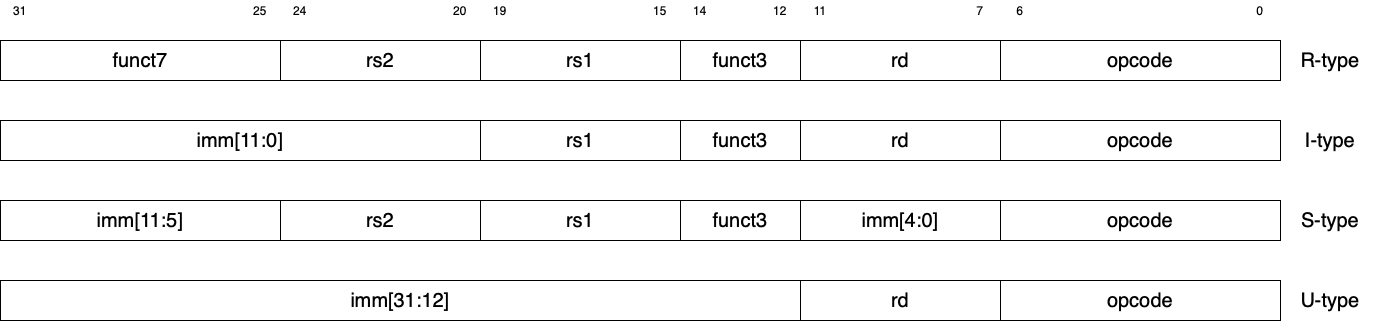
\includegraphics[scale = 0.27]{Chapter_1/img/riscv-base-instruction-formats.png}
    \caption{RISC-V base instruction formats. \cite{RISC-V-Instruction-Set-Manual}}
    \label{riscv-base-instruction-formats}
\end{figure}

It is important to notice that RISC-V is a load-store architecture, this means only load and store operations can have access to the memory.\\
It is a very convenient organization, because it reduces the average time-per-operation and guarantees a good functioning of the pipelined structure.\\

It also supports signed byte and half word loads, which is very useful when  working with signed byte and half word data types.

In Figure \ref{riscv-load-store} it is possible to see how the load-store instructions are composed, and that the LOAD is a I-type op and the STORE is an S-type op.

\begin{figure}[H]
    \centering
    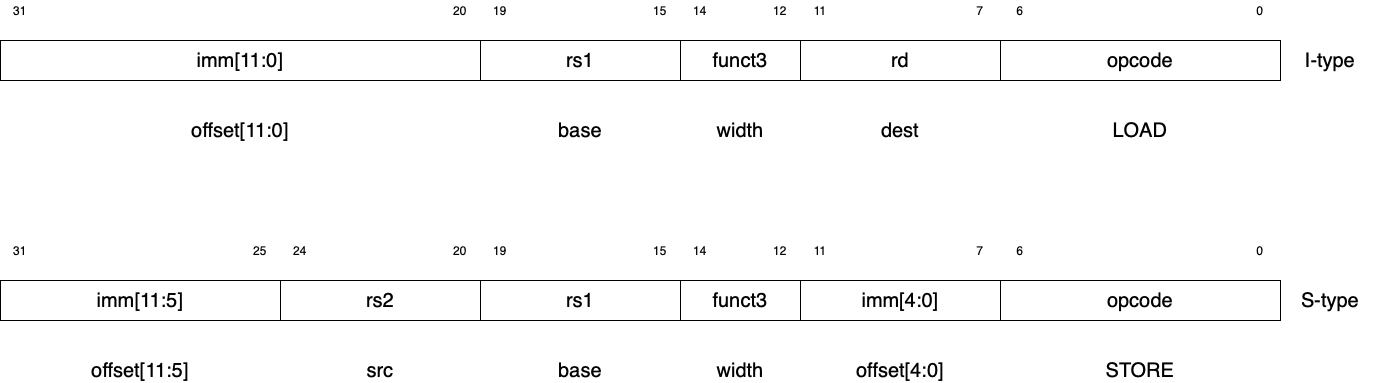
\includegraphics[scale = 0.27]{Chapter_1/img/riscv-load-store.png}
    \caption{RISC-V load/store instruction formats. \cite{RISC-V-Instruction-Set-Manual}}
    \label{riscv-load-store}
\end{figure}


\subsection{Parallel architectures, Vectors and RISC-V V-Extension}
In the last years the parallel architecture are gaining inertia on the processors field. This is happening because the real world has parallel behaviour and so the hardware we use to compute simulations and calculus needs to be.\cite{Parallel-Computing}\\
But why now and not before?\\
In the past, parallel computing efforts have shown promise and gathered investment, but in the end, uniprocessor computing always prevailed, what is different now?\\
Well, most of the paradigms that led to the unicore decision are now changing quickly as the technology changes its needs.\\
As the technology scales down to the nanometers, the power consumption and the energy consumption are becoming a problem, instead the cost of a single transistor is significantly lower.\\

But the multicore solution still doesn't meet the conformity for old binaries compilations and it could be difficult to program. So the solution of a parallel architecture with "manycores" seems to be the right one.\\

For this reason the vectors are useful. They allow to compute data in a parallel way, without having multicore programming logic.\\
A classic example are the VPU (Vector Processing Units) working with SIMD (single instruction multiple data).\\

A famous example of a vector architecture is the Cray-1. It was presented in 1975, and was a load/store architecture, as seen before.
It was designed for Supercomputing and the major feature was to have also a scalar mode. This because the vector computation is not always useful.\\

\subsubsection{Time efficiency}
As it is possible to see in Figure \ref{Multithreading} with standard multithreading there will always be some empty thread along with the running ones. This lowes the efficiency.
\begin{figure}[H]
    \centering
    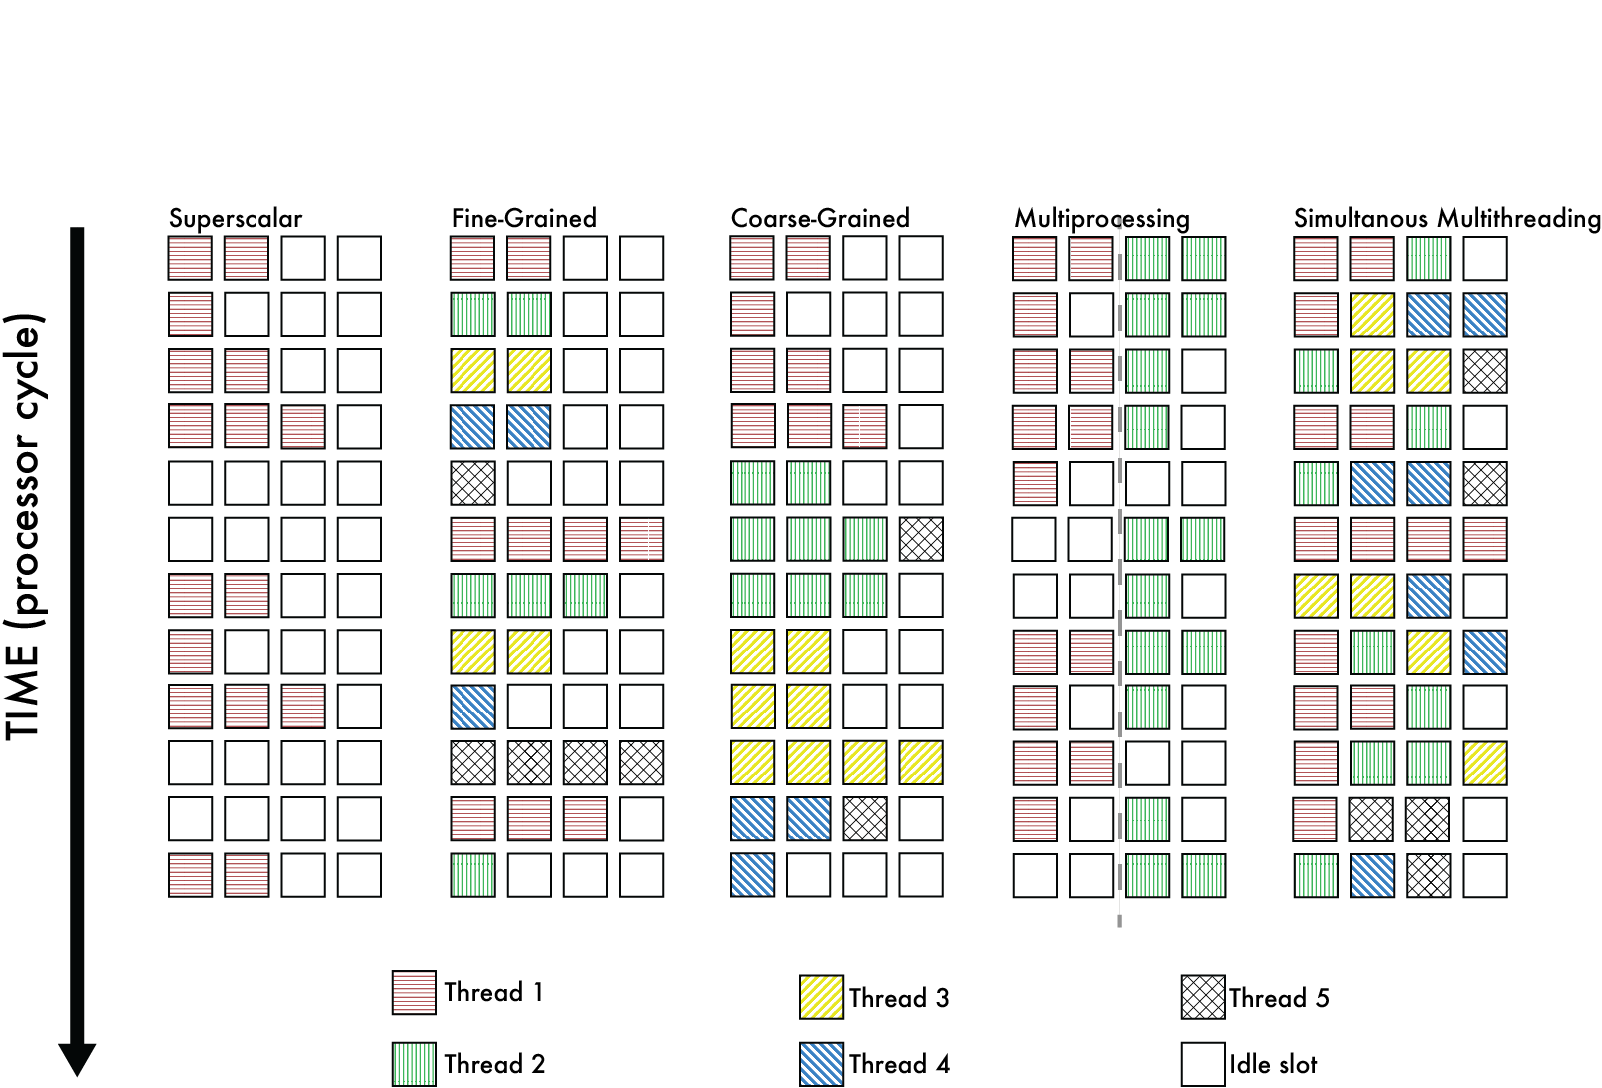
\includegraphics[scale = 0.5]{Chapter_1/img/threads.png}
    \caption{Multithreading Processor Clock Time usage  \cite{L15-Krste}}
    \label{Multithreading}
\end{figure}

Indeed the major advantage with the Vector computation is the condensation of the processor usage. 
So the usage will not be distributed as for standard multithreading processors, but it will have full usage for some cycles and zero usage for others\cite{L15-Krste}.\\

But of course there is a drawback, in particular the Latency. In vector computing there are always some dead cycles, but this also allows to increase the efficiency with modern low-power techniques, if it is possible to decrease the energy usage during the dead time.
The pipeline is represented in Figure \ref{Vector-Latency} and the final Clock Tima usage is represented in Figure \ref{Vectoring}.

\begin{figure}[H]
    \centering
    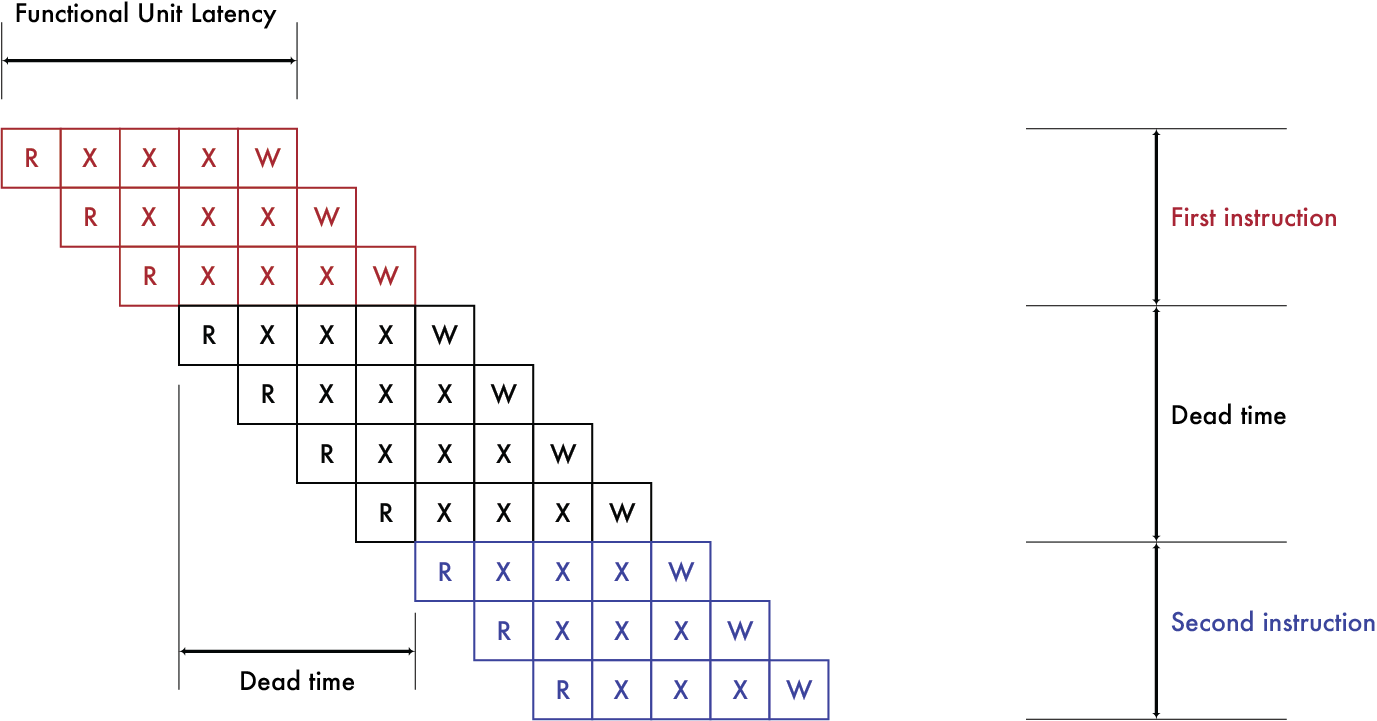
\includegraphics[scale = 0.5]{Chapter_1/img/lat-pen.png}
    \caption{Latency penalty on vector processing units \cite{L15-Krste}}
    \label{Vector-Latency}
\end{figure}

\begin{figure}[H]
    \centering
    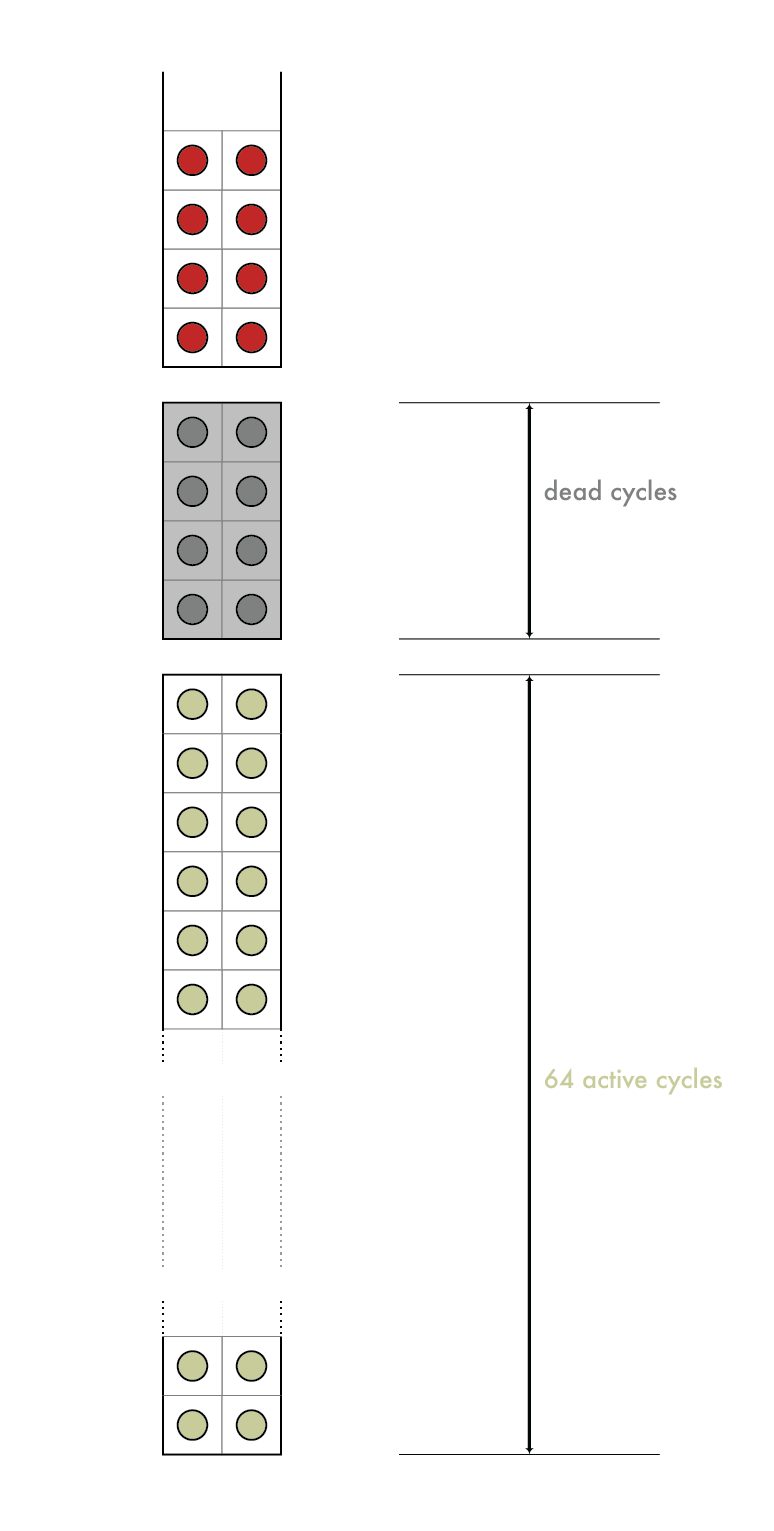
\includegraphics[scale = 0.35]{Chapter_1/img/time-usage.png}
    \caption{Vector Processor Clock Time usage \cite{L15-Krste}}
    \label{Vectoring}
\end{figure}
The RISC-V solution is V-Extension (V stands for Vector), and is in current development, in this thesis the reference will be the V-Extension 0.7.1.

The vector extension adds 32 vector registers, and five unprivileged CSRs (vstart, vxsat, vxrm, vtype, vl) to a base scalar RISC-V ISA\cite{riscv-v-specs}.
There are also 8 vector predicate registers (vp0-vp7). The CSRs vectors define the configurations.

\begin{table}[H]
    \centering
    \begin{tabular}{|l|l|l|l|}
        \hline
        Address & Privilege & Name   & Description               \\ \hline
        0x008   & URW       & vstart & Vector start position     \\ \hline
        0x009   & URW       & vxsat  & Fixed-point Saturate Flag \\ \hline
        0x00A   & URW       & vxrm   & Fixed-Point Rounding Mode \\ \hline
        0xC20   & URO       & vl     & Vector length             \\ \hline
        0xC21   & URO       & vtype  & Vector data type register \\ \hline
    \end{tabular}
    \caption{RISC-V's CSRs}
    \label{CSRs}
\end{table}

Based on the base scalar ISA and on the extensions implemented the datatypes and operations supported by the V extension change and they can be 16-bit, 32-bit, 64-bit, and 128-bit floating-point types or fixed-point types (F16, F32, F64, and F128, or X8, X16, X32, X64, and X128 respectively) \cite{riscv-v-specs}.\\


The vector unit must be configured before use. 
The active vector length is held in the CSR vl, which can only hold values between 0 and MVL inclusive.
The active vector length is usually written with the setvl instruction.\\

\subsubsection{Vector instructions}
Other than the base instruction we can expect from a Vector Architecture (as a move, add, xor and so on) it is possible to find some useful operations related to the nature of the vector calculus\cite{riscv-v-specs}:
\begin{itemize}
    \item \textbf{vectorial load/store}: those can strided or indexed. The strided ones index the elements referring to a starting one and then adding (or subtracting) a certain stride. This kind of load/store is very fast, in particular in some special cases (as unit-strided or some optimized power of 2).\\
    The elements into the indexed ones are basically pointed with an index. This process really slows down the operation but allows to select directly the elements.
    
    \item \textbf{widening/narrowing}: those operation are used to increase or decrease the size of the vector's contents, in fact they are very useful when performing operations that need to increase the result size (as example a multiplication between to integer at 32 bit needs to have 64 bit to not loose information). There are also few operations that require the inverse resizing, so the narrowing.
    
    \item \textbf{gather}: those are very particular operations and very useful when manipulating vectors. They allow to index a vector using another vector as index. In this way various patterns are possible.
    
    \item \textbf{reduction}: finally the reduction can perform an operation between a scalar and a vector and give as result a scalar (an easy example could be to calculate the maximum value between all the value contained in a vector and one scalar, the result would either be one of the element of the vector or the scalar).
    
\end{itemize}


Finally all those operations can be \textit{masked}. The masking is a common operation when there is branching or when complex patterns emerge.
Normally one bit of the mask represent a whole work or byte into the vector. Then an AND op is performed to have the final result. 

\subsection{Verification}
As the technology scales down, the design complexity explodes. 
Very small form factor have conflicting requirements for high performance, low-power and area constraints. 
This lead to a complex design and to elevate the costs of it.\\

It is possible to see in Figure \ref{verification-tecnology} how the cost for verification increases drastically with the lowering of the technology node.


\begin{figure}[H]
    \centering
    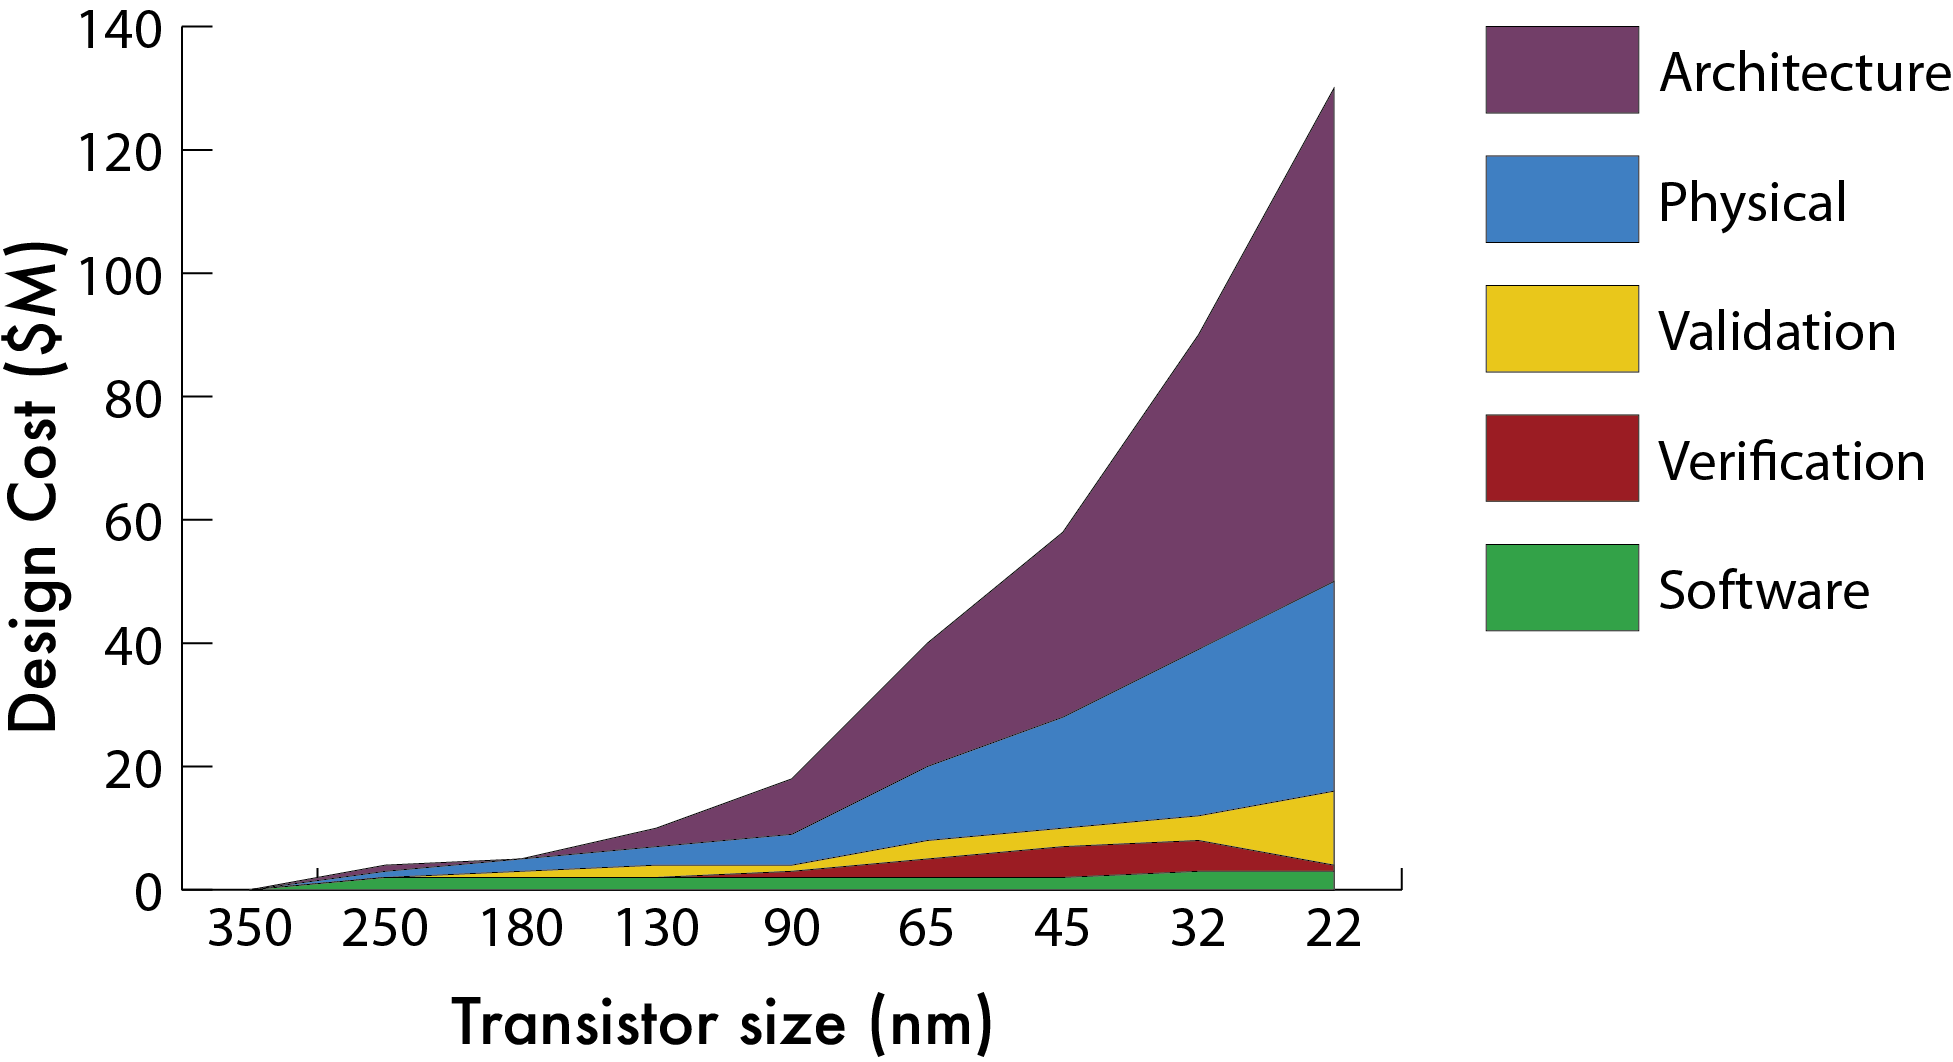
\includegraphics[scale = 0.4]{Chapter_1/img/cost-scale.png}
    \caption{Verification cost vs technology node \cite{verification-book-2018}}
    \label{verification-tecnology}
\end{figure}

the verification is responsible to make sure the design is in track with the specification, so as the design complexity increases so does the verification.\\

This is of course an issue for the time-to-market. 
In particular functional design verification takes 40–50\% of the project resources. In other words, increase the productivity of functional design verification and shorten the design / simulate / debug / cover loop is an essential task \cite{verification-book-2018}.\\

Also the compounded complexity grows faster that the compounded productivity. This gap only means the verification needs to be faster and so need to implement more techniques.
It is possible to see a study on the complexity/productivity gap in Figure \ref{complexity-gap}
\begin{figure}[H]
    \centering
    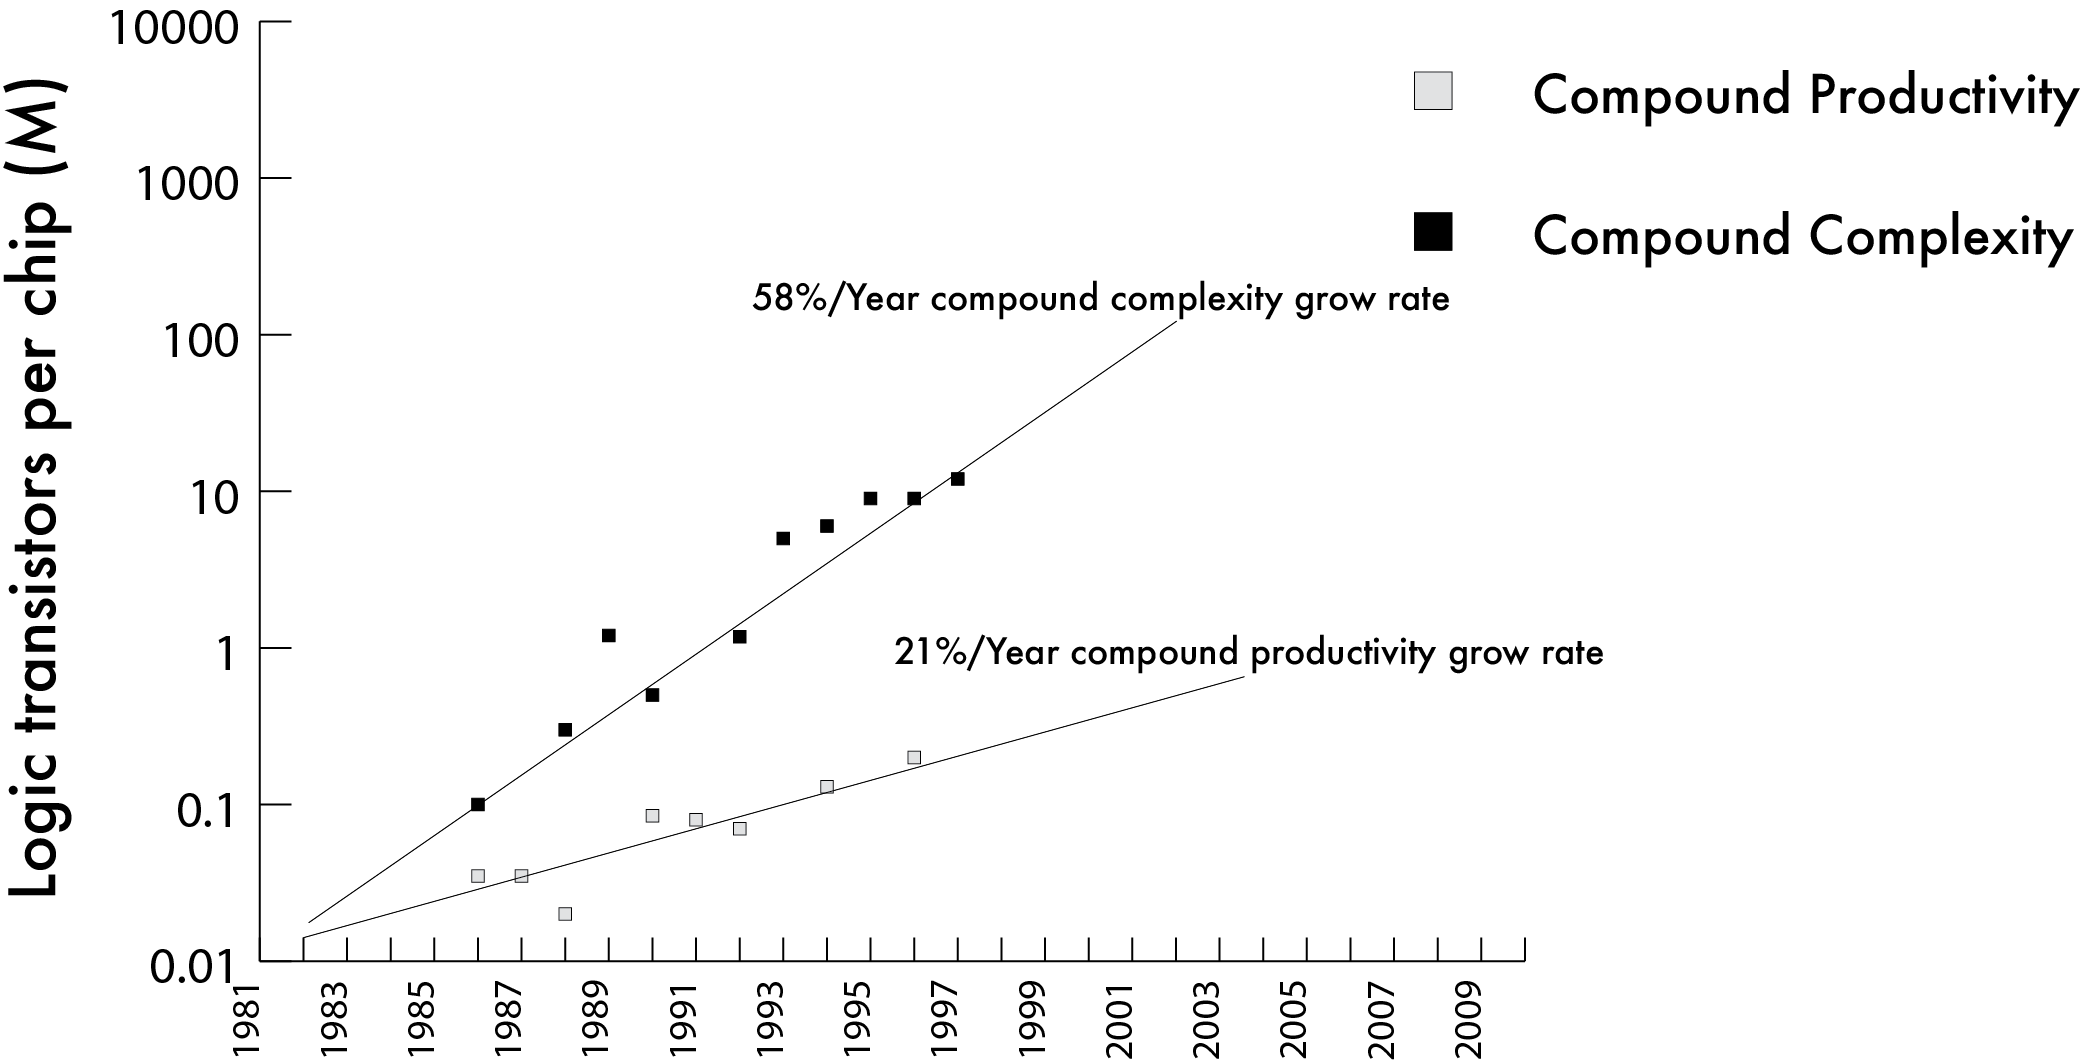
\includegraphics[scale = 0.4]{Chapter_1/img/prod-compl.png}
    \caption{The gap between the complexity and the productivity \cite{verification-book-2018}}
    \label{complexity-gap}
\end{figure}

\subsubsection{Verification approaches}
The verification mainly is divided in Functional and Formal verification:
\begin{itemize}
    \item \textbf{Functional}: it need to verify if the functionalities described into the specifications are met into the design. To verify functionally it is needed to define the functionalities and write them as code (normally checkers or scoreboard). This is a very important part of the process, as this translation is never perfect and often highlights some critical point into the specs.
    
    \item \textbf{Formal}: the formal verification can be done in different ways as \textit{model checking}, \textit{equivalence checking} and \textit{theorem proving}. \textit{Theorem proving} tries to prove the equivalence between specs and design using mathematical reasoning. \textit{Model checking} is useful when performing optimization to the design, trying to demonstrate the various versions are mathematically equivalent. Finally the \textit{model checking} is used to try to find counter example on the behaviour of the design, and in case simulating the specific case to demonstrate the falsity.
\end{itemize}

\bigskip

\subsubsection{Coverage}
The whole process of verification need also to have a direction. For that is used Coverage. \\

Coverage is very useful and can be performed on functionalities or on the code:
\begin{itemize}
    \item functionality: it measure the cover of all the functionalities stated by the specs. In this way it is possible to assure all the requirements are met. But this also means there is no information about not used RTL.
    
    \item code: it measure the cover of all the code. This means it is possible to know if there is unused code and possibly some branch of the flow. This also means there is no check about the functionalities implemented.

\end{itemize}

Trying to take the coverage to 100\% is the main goal. But at the same time it is easy to fool the coverage. This because it depends on how the cases are taken into account. \\

To be able to use all those techniques there is the need of a structure to contain and control them.
This structure is called \textit{UVM}, and it is formed by different classes useful to instantiate the controls and the drivers needed to verify the RTL. It will be discussed the particular case of this work later on this Chapter.

\section{Context}
%%%%%%%%%%%%TODO%%%%%%%%%%%%
%%%%%%%%CHECK AVISPADO%%%%%%%%
Before starting it is important to notice in this project it is not used the RISC-V scalar core to test and develop the VPU, instead it is used a simulator of it. The simulator is called Spike, and the core is called Avispado. Spike is also used for other tasks, so the Avispado simulation will always be called Avispado.\\
In Figure \ref{avi-vpu} it is possible to see the interface between Avispado and the VPU for all the instructions.\\
%%TODO correction to the palette
\begin{figure}[H]
    \centering
    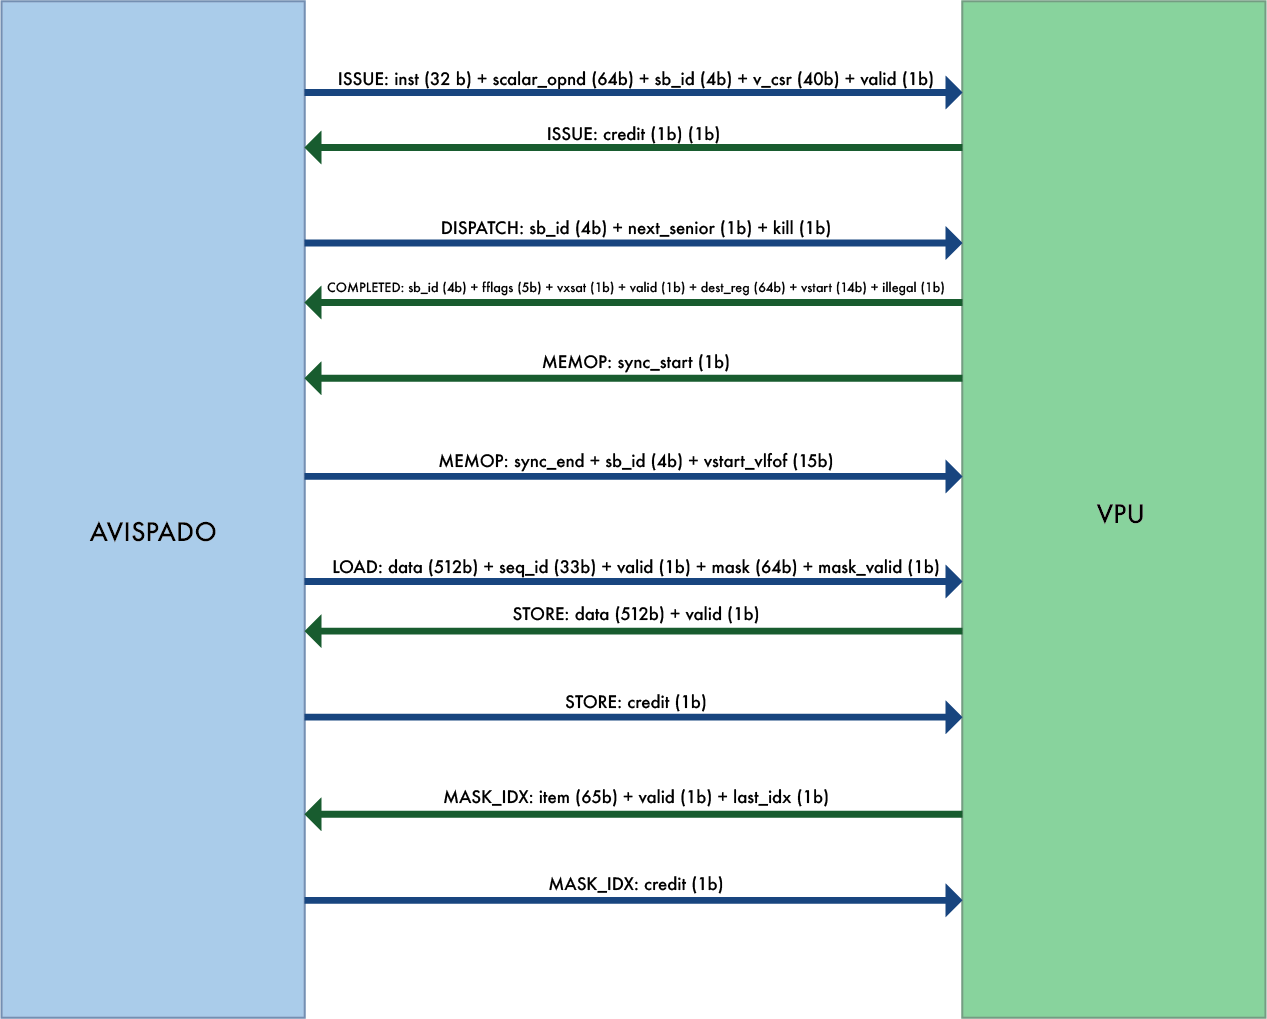
\includegraphics[scale = 0.6]{Chapter_1/img/avi-vpu.png}
    \caption{Avispado-VPU interface}
    \label{avi-vpu}
\end{figure}


The instructions are issue with a credit system, which number corresponds to the  depth of the issue queue of the VPU.\\

The handshake and the interface will be discussed later on when considering mostly the VPU side.



\subsection{The VPU}
In Figure \ref{VPU} it is possible to find a simplified scheme of the implemented VPU.\\

\begin{figure}[H]
    \centering
    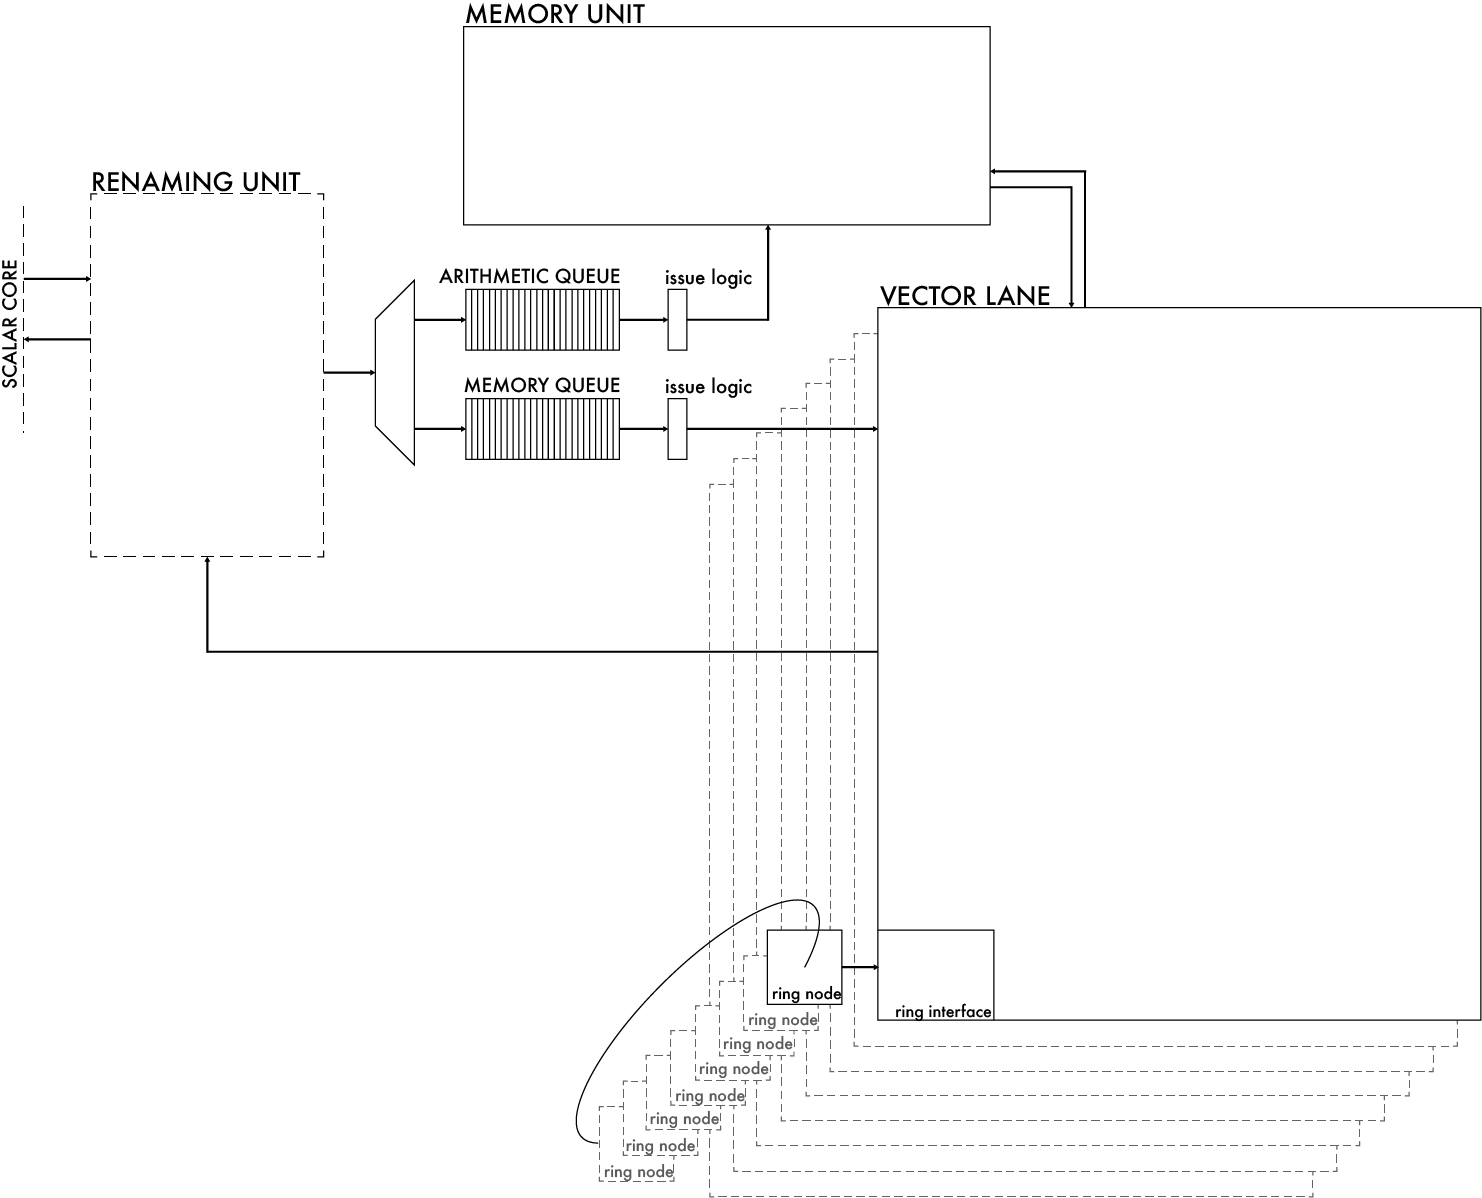
\includegraphics[scale = 0.5]{Chapter_1/img/VPU.png}
    \caption{EPI project's VPU}
    \label{VPU}
\end{figure}
It is important to notice the VPU implemented is able to work in an out-of-order way. This means the instructions can be executed not in order and then committed in order.\\


The main elements componing the VPU are:
\begin{itemize}
    \item \textbf{Renaming Unit}: the scope of this unit is to remove false dependeces due to the naming of the registers. This is possible because of the virtual memory, so the processor only uses logical registers, but in this component they are mapped to physical registers using the FRL (Free Register List).\\
    Then this translation is tracked into the RAT (Register Alia Table) in this way the logical source register, reading the RAT, can refer to the physical register.\\
    The last optimization is performed trying to remove the write-to-write dependencies and so avoiding also Data Hazards.\\
    When a physical register is not useful anymore, it is pushe to the FRL at commit time.
 
    \item \textbf{Queues}: the VPU is a decoupled vector architecture, this means that the arithmetic instructions and the memory instructions are buffered in different queues.\\
    In this scheme is possible to see how the 2 queues are independent in the issue stage, in which the instructions are sent respectfully to the vector lanes or the memory unit.\\
    The vector lane is capable to perform only one arithmetic instruction at time, so the issue queue must wait  until the previous instruction finishes its execution, but at the same time a memory instruction can be performed.\\
    The whole Issue stage is composed by the queue and the issue logic. The number of entries in the issue queues is parameterized.
    
    \item \textbf{Memory Unit}: as said before, the only instructions that can access the memory are the load and the store operations. The MU receives those instructions by the memory queue and it can only perform one instruction at time. 
    The possible addressing modes are unit-strided, strided and indexed.\\
    
    The memory requests are performed in order. This means there is a FIFO containing all the requests containig the useful informations as memory address, VL and stride.
    It is also checked if the same request is performed more times.\\

    There are different configurations that can be used, configuring the connection between the vector memory port and the CPU.
    It is also possible to bypass the first level of cache or to set the parameter of the MSHRs (miss status holding registers), which can be useful for large vector implementations.

    
    \item \textbf{Vector Lane}: the Vector Lane is the core of the VPU and operates on the vector register file. It is composed by different vector processing lanes. This is a very common technique that allows to improve performance and scalability.\\
    In an ideal multi-lane vector architecture all the lane are working simultaneously and so efficiently, with the cost of more hardware to control the synchronization.\\
    
    One of the most important submodules of the Vector Lane is the VRF (Vector Register File). This is designed with only one read/write port, this because it is important to limit the area usage, and so the operating frequency.
    To avoid streaming problems and bubble inside the pipe is so necessary to have a buffer.\\
    
    This solution also means there is some cost in terms of latency, due to the starting of a new instruction.
    Inside the Vector Lane are also important the WB (Write-Back Buffer) and the LB (Load Buffer). Those buffers store the data until the VRF line is complete.\\
    Then there is the SB (Store Buffer) which hold the data read from the  register file and then sends it to the MU. 
    Eventually when an instruction is completed the physical register are then freed. 
    
    The VPU can be configured with different numbers of lanes from 1 up to 8, the default value is 8.\\
    
    \item \textbf{Lane Interconnection}: because the Lanes can be any value between 1 and 8 is important to have a system which can synchronize all of them. There are also some operations which require to use multiple lanes at once to perform the execution, so a bidirectional ring intercommunication is implemented between the lanes.
\end{itemize}

It is also important to know how the memory is organized in order to understand how some operations work.\\

The vectors are distributed into the different lanes. Indeed it is possible to say the Vector are sliced into the lanes, this means it is necessary an efficient organization in order to understand where put the right data.\\


According to the RISC-V V-extension, vector elements can have different sizes. The parameter that describes the size of an elemetn is the SEW (Standard Element Width). This is determined by the CSR (Control and Status Register) named vsew. The maximum supported SEW into the EPI project is 64 bits. Also the maximum VLEN is equal to 16384 bits, so 2kB.\\

Considering the constraint of at least 40 physical registers, the number of lanes is equal to 8.
The number of elements a vector registers holds is given by VLEN/SEW, according to the Table \ref{sew-el}:


\begin{table}[H]
    \centering
    \begin{tabular}{|l|l|}
    \hline
        \rowcolor[HTML]{C0C0C0} 
        SEW & ELEMENTS \\ \hline
        64  & 256      \\ \hline
        32  & 512      \\ \hline
        16  & 1024     \\ \hline
        8   & 2048     \\ \hline
    \end{tabular}
    %\caption{Caption}
    \label{sew-el}
\end{table}

In Figure \ref{vrf-64} it is possible to see the structure used for SEW = 64 bit as examples.
\begin{figure}[H]
    \centering
    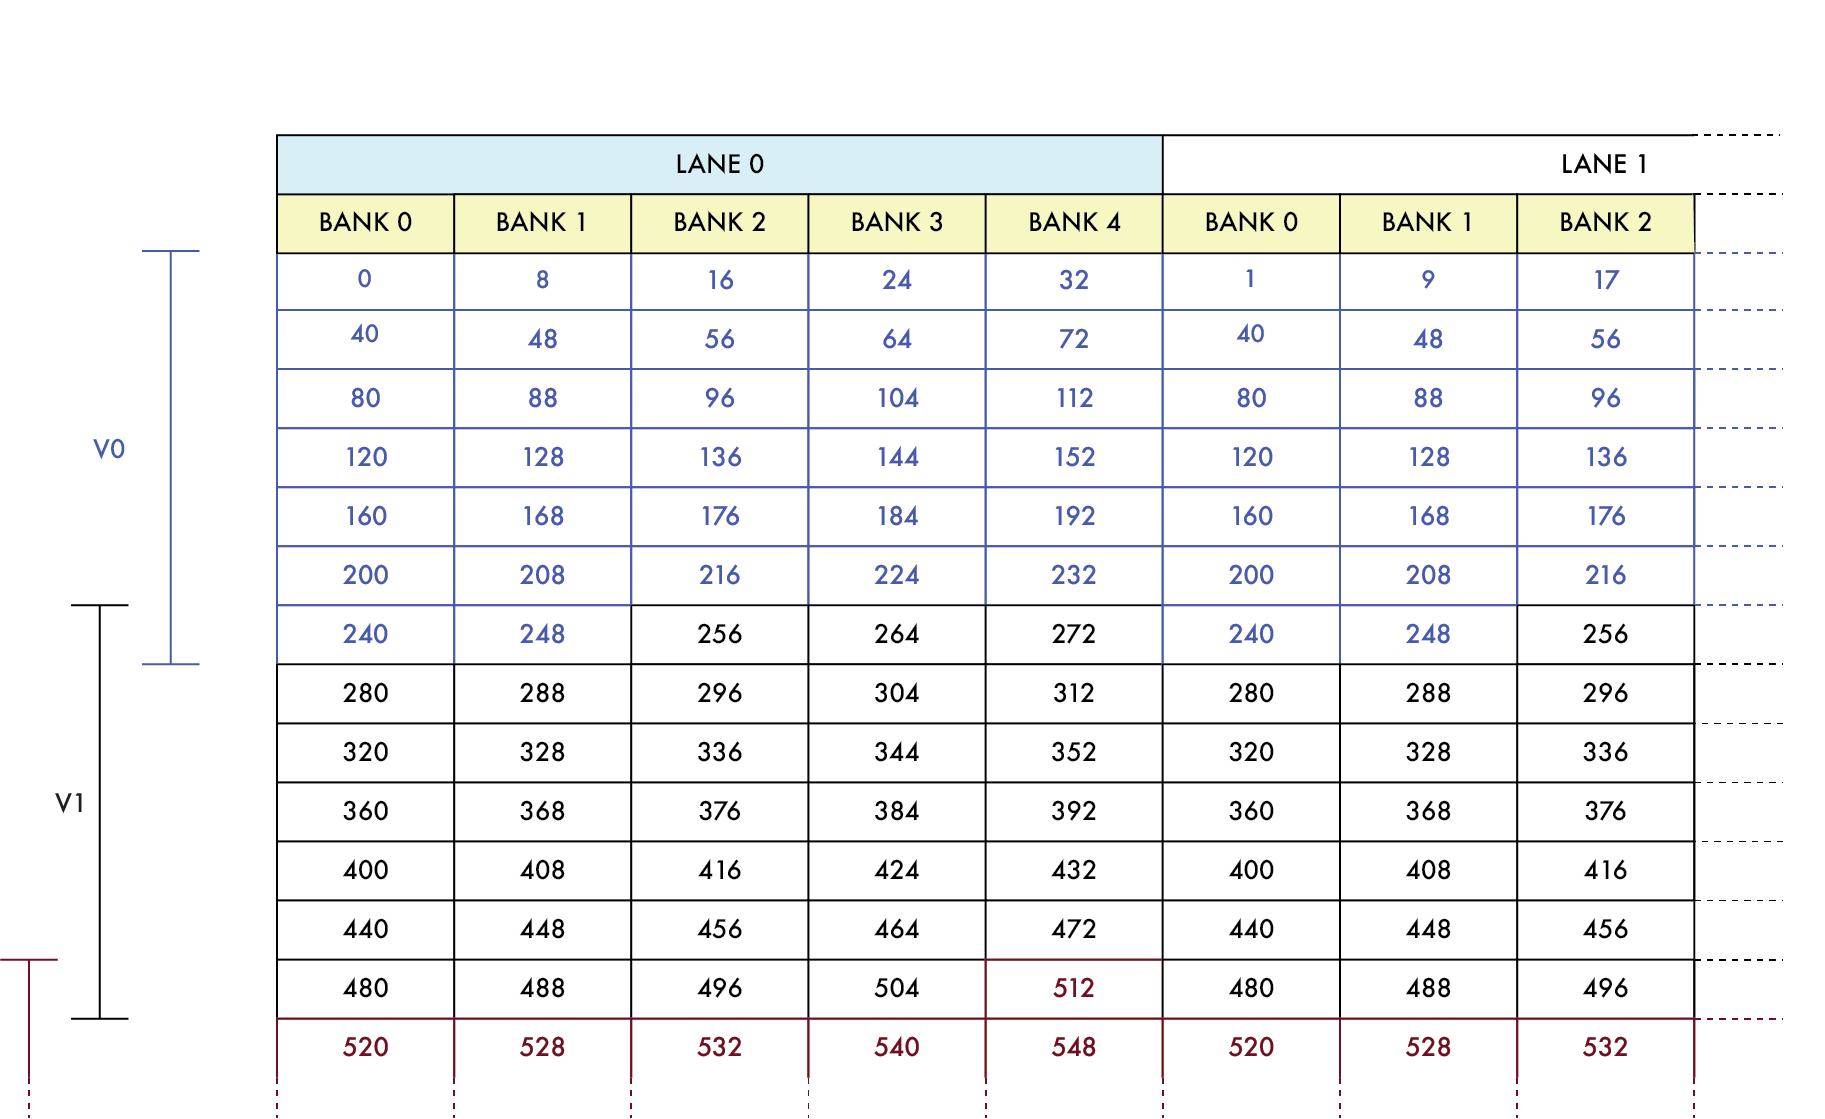
\includegraphics[scale = 0.45]{Chapter_1/img/vrf-64.png}
    \caption{VRF with sew = 64}
    \label{vrf-64}
\end{figure}

Notice that the sub-banks are more than 1 only when the SEW is not 64. \\

In Figure \ref{vrf-32} it is possible to identify the sub-banks as subdivision of a bank when SEW is not 64.
\begin{figure}[H]
    \centering
    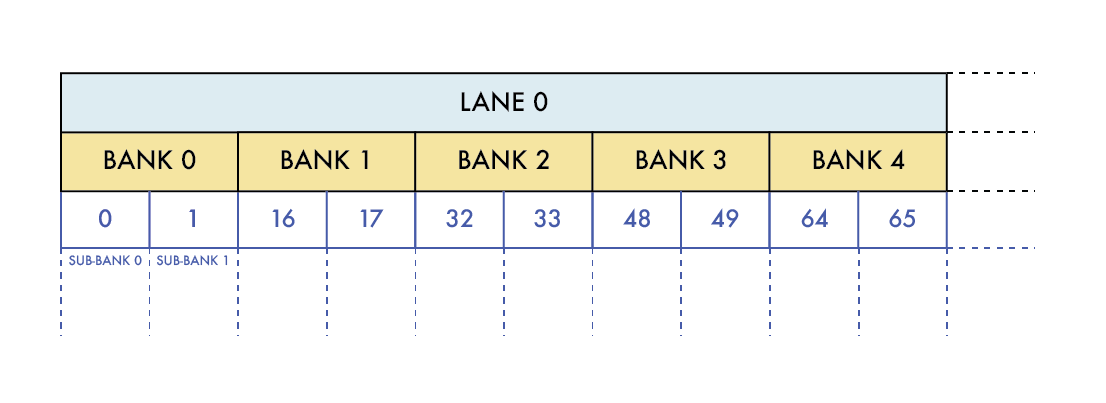
\includegraphics[scale = 0.7]{Chapter_1/img/vrf-32.png}
    \caption{VRF with sew = 32}
    \label{vrf-32}
\end{figure}

Let's focus now on the submodules on which the work of this thesis was done.




\subsection{The UVM}
As mentioned before, the UVM is the solution to the standardization problem of the verification. In fact it is is a transaction-level methodology (TLM) designed for testbench development. It is a class library that makes it easy to write configurable and reusable code \cite{verification-book-2018}.

The testbenches created are designed to be reusable, in this way less code and more production is achieved.\\

This is mainly obtained with the polymorphism. It means an object can be used to define a reusable class. In this way an object can be used as a super-class and other sub-classes can be done by that.\\

It works following an hierarchy method, and every component can only operate with the components above it. In this way multiple subcomponents can be instantiated.\\

\subsubsection{Generic UVM}
In Figure \ref{gen-uvm} it is possible to see an example of a standard UVM.

\begin{figure}[H]
    \centering
    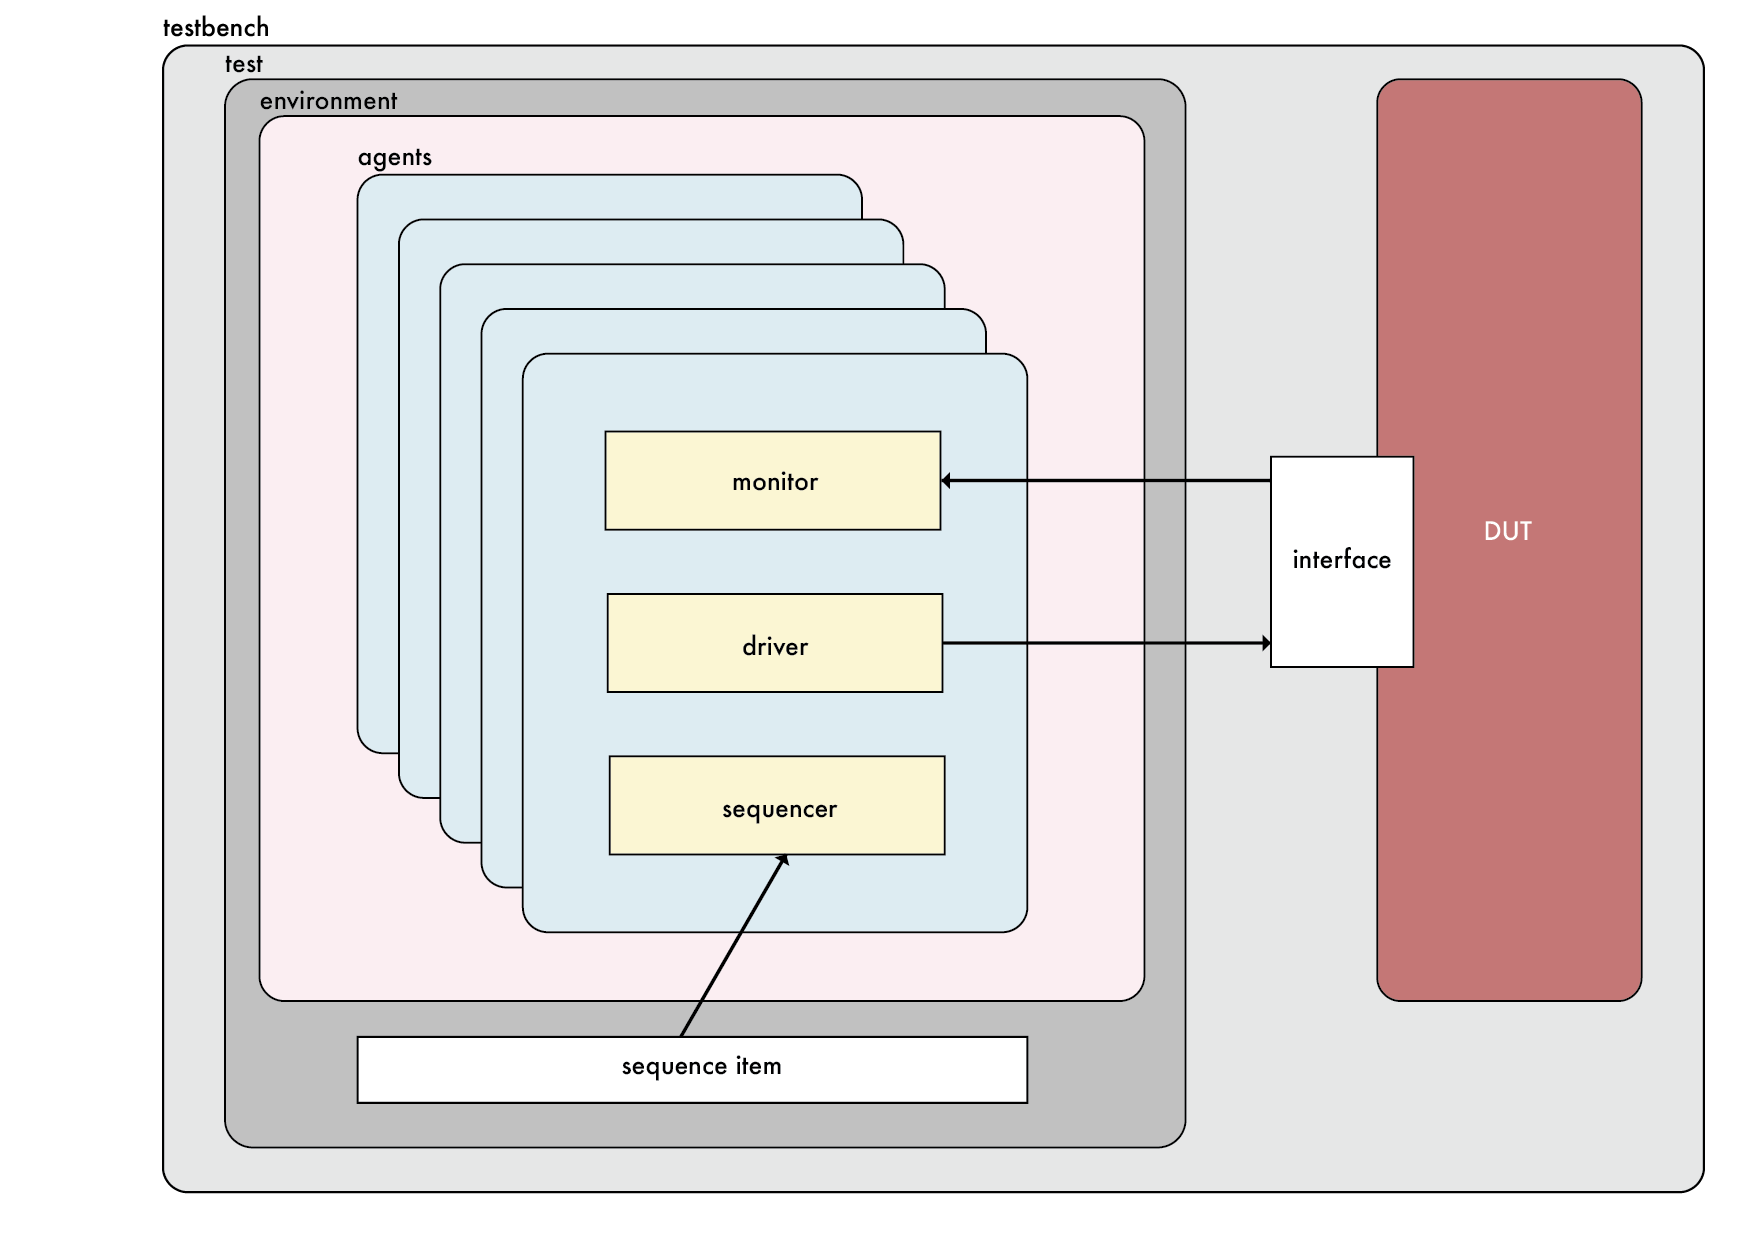
\includegraphics[scale = 0.4]{Chapter_1/img/general-uvm.png}
    \caption{A generic UVM}
    \label{gen-uvm}
\end{figure}

Let's now analyze some elements of a standard UVM and its implementations in the EPI project.

\begin{itemize}
    \item \textbf{Testbench}: typically it instantiates the DUT (Design Under Test) and the UVM Test Class. Also it is responsible to configure the connections between them.\\
    There are different ways to communicate into an UVM and in this module is possible to choose them.\\
    It is also important to say the Testbench instantiates the Test dynamically at run-time, in this way it possible to compile it once and run many Tests.
    
    \item \textbf{Test}: this is the top-level component into an UVM testbench.\\
    Typically a base test class is defined to instantiate the top-level environment and then it is extended to the specific case.
    
    \item \textbf{Environment}: it is a component that defines the environment of a test. This means to define all the agents and the scoreboards. 
    The top-level environment instantiates and configures the reusable verification IP and defines its default configurations based on the application of the test.\\
    
    Typically there is different environment for each interface of the DUT.
    
    \item \textbf{Sequence Item}: it is the fundamental lowest denominator object in the UVM hierarchy. It can be defined also as a transaction and is the smalles data transfer tha can exist in a UVM. It can inclued variables and constraints.\\
    
    It doesn't work with bits or those kind of astractions useful only when working with the DUT.
    
    \item \textbf{Sequence}: it is generated by the environment using the sequence item. It is an ordered collection of transactions.\\
    Mostly it can impose some contraint to the variables generated into the sequence item.
    
    \item \textbf{Agent}: it is one of the most important components of the UVM. It groups toghether a the components that are dealing with the DUT and so a specific DUT interface.\\
    Normally there is a different agent for every interface or DUT. This allows specific sequencers for specific stimulus.\\
    It can also be active or passive depending on its action on the DUT: if it sends signal to stimulate the DUT it is considered active, and otherwise passive.
    
    It contains:
    \begin{itemize}
        \item \textbf{Driver}: it is the component in charge to communicate between the UVM and the DUT at pinlevel. It receives the sequences from the sequencer and then converts them into signals, following the interface protocol.\\
        This action is observed by another component, the (command) monitor.
        It could monitor the data by itself by this would violate the modularity choices for the UVM.\\
        
        It can be turned off when the agent is defined as passive. In this way there is no other component sending signals to the DUT.

        
         \item \textbf{Sequencer}: it controls the requests and the responses between the driver and the sequence item. So it is a controller.
         
        \item \textbf{Monitor}: it controls the outputs of the DUT at pinlevel. Then transforms those signals into transactions for the analisys.\\
        It is also possible those transactions are then compared with the expected outputs. This is normally done in the scoreboard.\\
        It can perform interally some processing. 

        
    \end{itemize}
    
    \item \textbf{Scoreboard}: it is a checker for the outputs of the DUT. It compares the transactions obtained by the monitors against a predicted result.\\
    There are different ways to generate a predicted result and so a scoreboard, it often uses a C/C++ model, but it is possible to use also other languages.
    
\end{itemize}


It is important to point the UVM works in different phases.\\
It is possible to macro-divide the process in 3 phases: the \textit{build phase}: here the components are constructed from the top; the \textit{connect phase}: here all the components are connected upwards; and the \textit{run phase}: in this phase the simulation is ran.

In Figure \ref{phases-uvm} it is illustrated a simple scheme representing all the phases.\\


\begin{figure}[H]
    \centering
    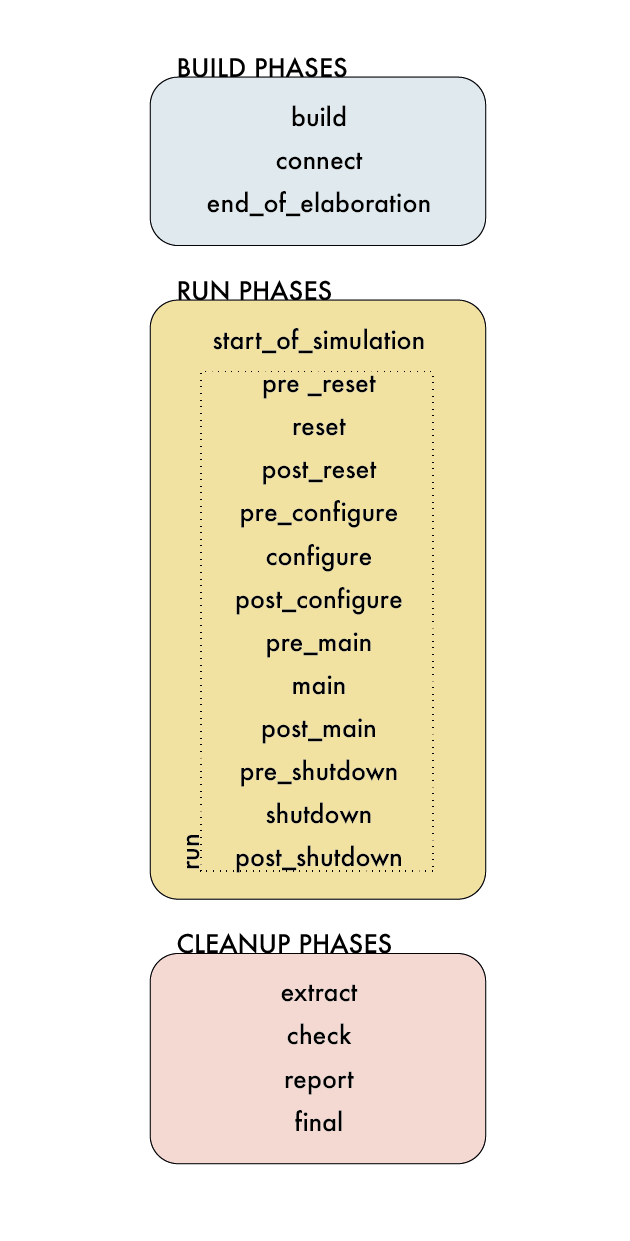
\includegraphics[scale = 0.6]{Chapter_1/img/phases-uvm.png}
    \caption{UVM phases}
    \label{phases-uvm}
\end{figure}


In this project two different UVMs were implemented. One to test of all the VPU and another one to test the submodules. This approach was chosen because it is not always obvious where a bug found is located.

Let's now analyze briefly those two structures.
\subsubsection{Main UVM}
The main UVM is interfaced with Avispado and it is composed following the standard structure. It was mainly used to support the use of a scoreboard (Spike) and to implement then some checkers and some coverage controls.\\

The majority of the automatic tests are made with this structure, and they are scripted to run all the night and to produce a valid dataset to then find and fix the bugs.\\

Using a simulator for Avispado as input, the driver is a little bit different from a standard one. Indeed the input are not controlled at pinlevel but vector instructions are sent to the core, which will then produce a correct input for the VPU.\\

Those instructions are then compared with with the scoreboard and a result is produced.

\subsubsection{Submodules UVM}

Another structure was necessary due to the different interface, and so different drivers. It is not always trivial to create a driver for a submodule, because the handshake processes can be very complex, and so it would be possible to introduce some error in the verification structure.\\

In this case this structure was used only for one submodule, and for the other one other techniques were implemented.\\

The structure of this UVM is represented in figure \ref{sub-uvm}. It was used mostly to handle the checkers and the drivers.

\begin{figure}[H]
    \centering
    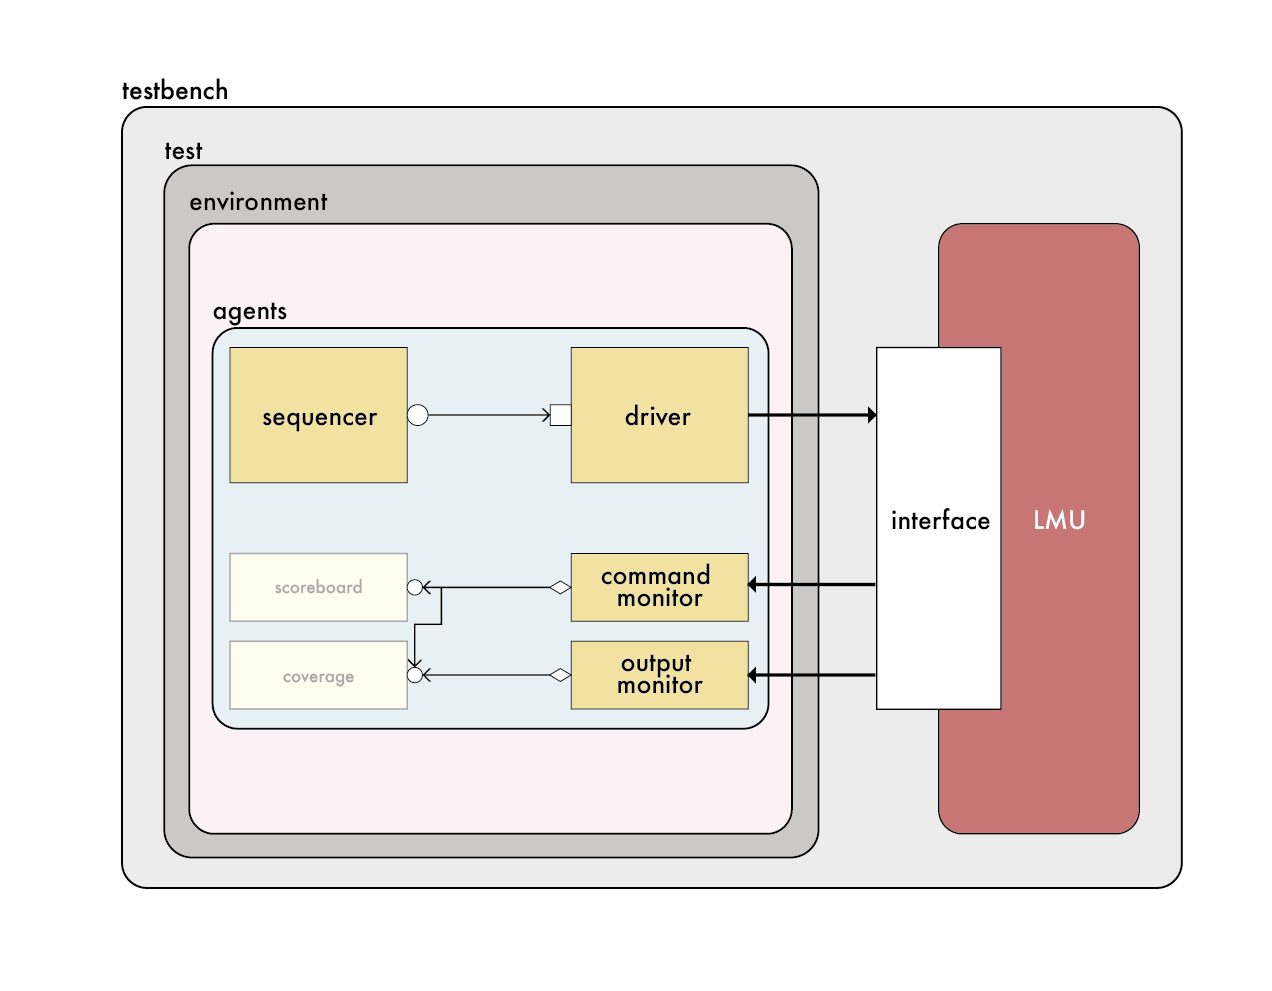
\includegraphics[scale = 0.5]{Chapter_1/img/sub-uvm.png}
    \caption{A small UVM for the submodules}
    \label{sub-uvm}
\end{figure}

It is possible to observe the scoreboard and the coverage are disabled in this application. In reality a scoreboard was implemented for each of them, but was handles with a different methodology discussed later on the next Chapter.